% Important: The shell-escape flag is required for the Minted package.
% Please compile this document with 'pdflatex -shell-escape main.tex'.
% If you are using another IDE, you may be able to specify this in the
% options or to provide an option like '% !TEX option = -shell-escape'
% in this file, depending on your builder. See the README.md for more.

% Don't put any content in here.
% Don't even include content files by using \input or \inlcude.
% Put your content into components/text.tex or include it there using \input.
% You probably want to modify the following files:
%   components/info.tex             contains the author, title etc.
%   components/settings.tex         contains the packages and settings.
%   components/commands.tex         contains helpful custom commands.
%   components/glossary.tex         contains an explanation of the used terms.
%   components/acknowledgements.tex contains the acknowledgements.
%   components/quote.tex            contains a quote.
%   components/abstract.tex         contains the abstract of the document.
%   components/text.tex             includes the actual content of the document.
%   components/outline.tex          contains the outline.
%   components/preface.tex          contains the preface.
%   chapters/                       contains the main text.
%   bibliography/literature.bib     contains the BibTeX entries.
%   images/                         contains all your content-related images.
%
% You probably don't need to change anything in the following files:
%   components/cover.tex            formats the front cover of the document.
%   components/titlepage.tex        formats the title page of the document.
%   components/disclaimer.tex       formats the disclaimer page.
%   styles/                         contains style elements (e.g. logos).
%   main.tex                        contains the top-level code structure.
%   README.md                       contains information about this template.

\documentclass[11pt,
              a4paper,
              article,
              index=totoc,
              headsepline,
              footsepline,
              BCOR=12mm,
              dvipsnames,
              DIV=13]{scrbook}
\setcounter{secnumdepth}{3}
\usepackage{amsthm}
\usepackage[ruled,vlined]{algorithm2e}
\usepackage{tikz}
\usepackage{wrapfig}
\usetikzlibrary{shapes,arrows,positioning}
\setlength{\parindent}{0pt}
\setlength{\parskip}{6pt}
\usepackage{caption}
\usepackage{subcaption}
\usepackage{adjustbox}
\usepackage{acronym}
\usepackage{hyperref}[2011/02/05]

\makeatletter
\AtBeginDocument{%
  \renewcommand*{\AC@hyperlink}[2]{#2}%
}
\makeatother

% KOMA scrbook options:
%  index=totoc: include an entry for the index in the table of contents.
%  headsepline: use horizontal line under heading.
%  footsepline: use horizontal line above footer.
%  BCOR: binding correction (e.g.: BCOR=12mm)
%  DIV: Number of sheet sections (used for layout) (e.g.: DIV=13)


%  This code base is currently hosted at: 
%  https://github.com/waltsims/TUM_Thesis_Template_CSE
\usepackage[backend=biber, sorting=none]{biblatex}
\addbibresource{bibliography/literature.bib}
% !TEX root = ../main.tex
% Set here the title, authors and other stuff to be used for the cover
% This file is used by MAIN.TEX

% set title, authors and stuff for the cover
\def\university{Technische Universit{\"a}t M{\"u}nchen}
\def\universityLogo{styles/tum_logo}
\def\program{Robotics, Cognition, Intelligence (M.Sc.)}
\def\programLogo{styles/cse_logo}
\def\doctype{Master's Thesis}

\def\title{A Noval Approach For Inference Time Search On Continuous Action Space in Deterministic Environments}
\def\author{Hendrik Elvers}
\def\supervisor{Prof. Dr.-Ing. habil. Alois Knoll}
\def\advisor{Dr. rer. nat. Zhenshan Bing}
\def\date{April 15th, 2023}

\def\keywords{{RL}, {IL}, {POMDP}}

% The following are used for the PDF metadata, by default the same as above.
\def\metaTitle{\title}
\def\metaAuthor{\author}
\def\metaSubject{\doctype\ -\ \university}
\def\metaKeywords{\keywords}

% text to appear in the footer
\def\footertext{}


% !TEX root = ../main.tex
% Included by MAIN.TEX

%--------------------------------------------------
% Fonts and page setup
%--------------------------------------------------

% Default font
\usepackage{palatino}

% Enable special PostScript fonts (optional)
% \usepackage{pifont}

% Manipulate the footer
\usepackage{scrlayer-scrpage}
\usepackage{scrhack}
\pagestyle{scrheadings}
\ifoot[\footertext]{\footertext} % \footertext set in INFO.TEX

% Set the font for the section headings
\renewcommand{\sectfont}{\normalfont \bfseries}

% Conditional commands in LaTeX documents, used for the \clearemptydoublepage.
\usepackage{ifthen}

% Typeset text in multiple columns (optional)
% \usepackage{multicol}

% Rotation tools, including rotated full-page floats (optional)
\usepackage{rotating}


%--------------------------------------------------
% Document structure
%--------------------------------------------------

% Pro­duce hy­per­text links in the doc­u­ment (recommended)
\usepackage{hyperref}

% Create glossaries and lists of acronyms
% depending on how many packages were shipped with your TeX distribution,
% you might need to install xindy. On Linux: sudo apt install xindy
\usepackage[toc, xindy]{glossaries}

% Standard LaTeX package for creating indexes
\usepackage{makeidx}


%--------------------------------------------------
% Bibliography
%--------------------------------------------------

% Set the bibliography style (default: plain)
\bibliographystyle{plain}

% Special biblography package (nice to have)
% \usepackage{natbib}


%--------------------------------------------------
% Graphics and floats
%--------------------------------------------------

% Enhanced support for graphics (recommended)
\usepackage{graphicx}
% Path to the figures directory (default: {figures/})
% Multiple entries are allowed, e.g. {{figures1/}{figures2/}}.
\graphicspath{{figures/}}

% Improved interface for floating objects (optional)
\usepackage{float}

% To use the subfigures (optional)
\usepackage{subcaption}


%--------------------------------------------------
% Mathematics
%--------------------------------------------------

% AMS mathematical facilities for LaTeX (recommended)
\usepackage{amsmath}

% TeX fonts from the American Mathematical Society (recommended)
\usepackage{amsfonts}

% Some extra math symbols (optional)
% \usepackage{amssymb}

% Extended maths fonts for LaTeX (optional)
% \usepackage{yhmath}

% Provide math delimiters whose size can be computed automatically (optional)
% \usepackage{commath}


%--------------------------------------------------
% Source code and algorithms
%--------------------------------------------------

% Source code typesetting
% \usepackage{listings} % (optional - alternative)
\usepackage[newfloat]{minted} % (recommended)
% Set global Minted options
\setminted{linenos, autogobble, frame=lines, framesep=2mm}
% Inline C++ (optional)
\newcommand{\incpp}[1]{\mintinline{c++}{#1}}
\newenvironment{code}{\captionsetup{type=listing}}{}
\SetupFloatingEnvironment{listing}{name=Source Code}

% Typeset algorithms - pseudocode (optional)
% \usepackage{algorithmicx}
% \usepackage{algpseudocode}
% Normal arrow comments
% \algrenewcommand{\algorithmiccomment}[1]{\hfill$\rightarrow$ #1}


%--------------------------------------------------
% Tables
%--------------------------------------------------

% Tables (optional)
\usepackage{tabu}

% Add color to LaTeX tables (optional)
% \usepackage{colortbl}

% Create tabular cells spanning multiple rows (optional)
% \usepackage{multirow}


%--------------------------------------------------
% Color
%--------------------------------------------------

% Use colors
\usepackage[dvipsnames]{xcolor}

% You may find all the pre-defined colors in
% https://en.wikibooks.org/wiki/LaTeX/Colors#Predefined_colors

% Custom colors
\definecolor{Pantone300C}{HTML}{0065BD} % TUM primary blue
\definecolor{Pantone301}{HTML}{005293}  % TUM secondary light blue
\definecolor{Pantone540}{HTML}{003359}  % TUM secondary dark blue
\definecolor{DarkGray}{HTML}{333333}    % TUM secondary dark gray
\definecolor{MediumGray}{HTML}{808080}  % TUM secondary medium gray
\definecolor{LightGray}{HTML}{CCCCC6}   % TUM secondary light gray
\definecolor{Pantone7527}{HTML}{DAD7CB} % TUM accent gray
\definecolor{Pantone158}{HTML}{E37222}  % TUM accent orange
\definecolor{Pantone383}{HTML}{A2AD00}  % TUM accent green
\definecolor{Pantone283}{HTML}{98C6EA}  % TUM accent very light blue
\definecolor{Pantone542}{HTML}{64A0C8}  % TUM accent light blue

% Color for the hyperlinks (e.g. table of contents)
\def\colorLinks{Pantone300C}
% Color for the web links
\def\colorUrl{Pantone542}
% Color for the citations
\def\colorCitations{Pantone158}

%--------------------------------------------------
% PDF output
%--------------------------------------------------

% Adjust the color of the links
\hypersetup{
  linkcolor=\colorLinks,%
  urlcolor=\colorUrl,%
  citecolor=\colorCitations
}

% Disable the coloring of the links when printing.
% Requires a compatible PDF reader.
\usepackage[ocgcolorlinks]{ocgx2}[2017/03/30]

% PDF Metadata
\hypersetup{
  pdftitle={\metaTitle},%
  pdfauthor={\metaAuthor},%
  pdfkeywords={\metaKeywords},%
  pdfsubject={\metaSubject}
}

% Create XMP Metadata (uses the values from hyperref)
\usepackage{hyperxmp}

% Make thumbnails (optional)
% \usepackage{thumbpdf}


%--------------------------------------------------
% Other settings
%--------------------------------------------------

% Define commands that appear not to eat spaces (optional)
\usepackage{xspace}


% !TEX root = ../main.tex
% Included by MAIN.TEX
% Please include your own cool commands here.
% Be only sure to comment it sufficiently so others can use it.

%-------------------------------------------------------------
%                      Own Commands
%-------------------------------------------------------------


%-------------------------------------------------------------
% math stuff -------------------------------------------------

% nice R, N, C
\newcommand{\nat}{\mathbb{N}}
\newcommand{\real}{\mathbb{R}}
\newcommand{\compl}{\mathbb{C}}

% un demi
\newcommand{\half}{\frac{1}{2}}

% parantheses
\newcommand{\parenth}[1]{ \left(#1 \right) }
\newcommand{\bracket}[1]{ \left[#1 \right] }
\newcommand{\accolade}[1]{ \left\{ #1 \right\} }
%\newcommand{\angle}[1]{ \left\langle  #1 \right\rangle }

% partial derivative: %#1 function, #2 which variable
% simple / single line version
\newcommand{\pardevS}[2]{ \delta_{#1} f(#2) }

% fraction version
\newcommand{\pardevF}[2]{ \frac{\partial #1}{\partial #2} }

% render vectors: 3 and 4 dimensional
\newcommand{\veciii}[3]{\left[ \begin{array}[h]{c} #1 \\ #2 \\ #3	\end{array} \right]}
\newcommand{\veciv}[4]{\left[ \begin{array}[h]{c} #1 \\ #2 \\ #3 \\ #4	\end{array} \right]}

% render matrices: 3  dimensional (arguments in row first order)
\newcommand{\matiii}[9]{\left[ \begin{array}[h]{ccc} #1 & #2 & #3 \\ #4 & #5 & #6 \\ #7 & #8 & #9	\end{array} \right]}

%-------------------------------------------------------------
% some abreviations ------------------------------------------
\newcommand{\Reg}{$^{\textregistered}$}
\newcommand{\reg}{$^{\textregistered}$ }
\newcommand{\Tm}{\texttrademark}
\newcommand{\tm}{\texttrademark~}
\newcommand {\bsl} {$\backslash$}

%-------------------------------------------------------------
% formating --------------------------------------------------

% Theorem & Co environments and counters
\newtheorem{theorem}{Theorem}[chapter]
\newtheorem{lemma}[theorem]{Lemma}
\newtheorem{corollary}[theorem]{Corollary}
\newtheorem{remark}[theorem]{Remark}
\newtheorem{definition}[theorem]{Definition}
\newtheorem{equat}[theorem]{Equation}
\newtheorem{example}[theorem]{Example}
%\newtheorem{algorithm}[theorem]{Algorithm}

% inserting figures
\newcommand{\insertfigure}[4]{ % Filename, Caption, Label, Width percent of textwidth
	\begin{figure}[htbp]
		\begin{center}
			\includegraphics[width=#4\textwidth]{#1}
		\end{center}
		\vspace{-0.4cm}
		\caption{#2}
		\label{#3}
	\end{figure}
}

% referecing figures

\newcommand{\refFigure}[1]{ %label
	Figure~\ref{#1}
}
\newcommand{\refChapter}[1]{ %label
	Chapter~\ref{#1}
}

\newcommand{\refSection}[1]{ %label
	Section~\ref{#1}
}

\newcommand{\refParagraph}[1]{ %label
	Paragraph~\ref{#1}
}

\newcommand{\refEquation}[1]{ %label
	Equation~\ref{#1}
}

\newcommand{\refTable}[1]{ %label
	Table~\ref{#1}
}

\newcommand{\rigidTransform}[2]
{
	${}^{#2}\!\mathbf{H}_{#1}$
}

% comment that appears on the border - very practical !!!
\newcommand{\comment}[1]{\marginpar{\raggedright \noindent \footnotesize {\textsl{#1}} }}

% page clearing
\newcommand{\clearemptydoublepage}{%
  \ifthenelse{\boolean{@twoside}}{\newpage{\pagestyle{empty}\cleardoublepage}}%
  {\clearpage}}

%-------------------------------------------------------------
%-------------------------------------------------------------

\newcommand{\etAl}{\emph{et al.}\mbox{ }}


% !TEX root = ../main.tex
\newglossaryentry{computer}
{
  name=computer,
  description={is a programmable machine that receives input,
               stores and manipulates data, and provides
               output in a useful format}
}

\newglossaryentry{poc}
{
  name={proof of concept},
  description={}
  }
\newglossaryentry{ui}
{
  name={user interface},
  description={}
  }
\newglossaryentry{ai}
{
  name={arithmetic intensity},
  description={a measure of floating-point operations (FLOPs)
              \hyphenation{per-formed} performed by a \hyphenation{gi-ven} given code or code section relative
              to the amount of memory accesses (Bytes) that are required
               to support those operations\cite{AI}}
  }

\newglossaryentry{speed-up}
{
  name={speed-up},
  description={the factor of temporal acceleration a program
  exhibits when additional computational resources are dedicated to it's execution.}
}

\newglossaryentry{directive pragmas}
{
  name={directive pragma},
  description={a computer programming language construct that specifies how a compiler
  should process input data} % sourced from wikipedia
}


\newglossaryentry{rc}{%SOURCE: wikipedia
name={race condition},
description={A race condition or race hazard is the behaviour of an electronic,
 software, or other system where the output is dependent on the sequence or
 timing of other uncontrollable events. It becomes a bug when events do not
 happen in the order the programmer intended. The term originates with the idea
 of two signals racing each other to influence the output first.}
}
\newglossaryentry{dd}{
name={data dependencies},
description={}
}
\newglossaryentry{sisd}{
name={single instruction single data},
description={}
}
\newglossaryentry{simt}{
name={single instruction multiple threads},
description={}
}

\newglossaryentry{simd}{
name={single instruction multiple data},
description={}
}
\newglossaryentry{gp}{%SOURCE: wikipedia
name={Gaussian Plane},
description={The two dimensional plane of complex numbers.}
}
\newglossaryentry{CURAND}{
name={CURAND},
description={
The CURAND library provides facilities that focus on the simple and efficient
generation of high-quality pseudorandom and quasirandom numbers.\cite{cuRAND}
}
}

\newacronym[longplural={partial differential equations}]{PDE}{PDE}{partial differential equations}
\newacronym{mpi}{MPI}{Message Passing Interface}

\newacronym[longplural={Random Walks on Spheres}]{RWoS}{RWoS}{Random Walk on Spheres}

\newacronym[longplural={graphical processing units}]{GPU}{GPU}{graphical processing unit}

\newacronym[longplural={central processing units}]{CPU}{CPU}{central processing unit}
\newacronym{hpc}{HPC}{high performance computing}

\newacronym[longplural={arithmetic logic units}]{ALU}{ALU}{arithmetic logic unit}

\newacronym[longplural={streaming multi-processors}]{SM}{SM}{streaming multi-processor}

\newacronym[longplural={boundary value problems}]{BVP}{BVP}{boundary value problem}
\newacronym[longplural={general purpose graphical processing units}]{GPGPU}{GPGPU}{general purpose graphical processing units}
\newacronym{CUDA}{CUDA}{compute unified device architecture}
\newacronym{RAM}{RAM}{random access memory}
\newacronym{SRAM}{SRAM}{static random access memory}
\newacronym{DRAM}{DRAM}{dynamic random access memory}
\newacronym{I/O}{I/O}{input/output}
\newacronym{PTX}{PTX}{Parallel Thread eXecution}
\newacronym{jit}{JIT}{just in time}


\makeglossaries

\begin{document} 

\begin{figure}
    \centering
    \begin{tikzpicture}
        \node[draw, fill=black!20, rounded corners, minimum width=2cm, minimum height=1cm] (planner) at (3,0) {$\text{Planner}_{t\rightarrow \color{black!50!green!80} t+1}$};
        \node[draw, fill=black!20, rounded corners, minimum width=2cm, minimum height=1cm] (critic) at (6,2) {Critic};
        \node[draw, fill=black!20, rounded corners, minimum width=2cm, minimum height=1cm] (actor) at (0,2) {$\text{Actor}_{t\rightarrow \color{black!50!green!80} t+1}$};
        
        \node[draw, fill=blue!20, rounded corners] (plans) at (0,0) {
            $\begin{cases}
                \begin{matrix}[p_1, ..., p_T\end{matrix} ]^\textbf{T}_{t>1}\\
                [0]_{t=1}
            \end{cases}$
            };
        \node[draw, fill=blue!20, rounded corners] (actions) at (3,2) {$\left[\begin{matrix}a_1\\ \vdots\\ a_T\end{matrix}\right]_t$};
        \node[draw, fill=blue!20, rounded corners] (exp_values) at (8.5,2) {$\left[\begin{matrix}c_1\\ \vdots\\ c_T\end{matrix}\right]_t$};
        \node[draw, thick, rectangle] (loss) at (11,2) {$|c^t_T - 1|_{_2}^{^2}$};

        \node[draw, fill=blue!20, rounded corners] (obs_1) at (0,5) {$\begin{matrix}[o_1,..., \times T, ..., o_1\end{matrix} ]^\textbf{T}$};
        \node[draw, fill=blue!20, rounded corners] (obs_2) at (6,5) {$\begin{matrix}[o_1,..., \times T, ..., o_1\end{matrix} ]^\textbf{T}$};

        \node[draw, thick, circle] (embplus_1) at (0,3.5) {$\oplus$};
        \node[draw, thick, circle] (embplus_2) at (6,3.5) {$\oplus$};

        \node[draw, thick, circle, inner sep=0pt,label={[align=left]left:Positional\\Encoding}] 
        (pe_1) at (-1.5,3.5) {\tikz \draw[scale=0.1] plot[domain=0.0:6.28] (\x,{sin(\x r)});};
        \node[draw, thick, circle, inner sep=0pt,label={[align=left]left:Positional\\Encoding}] 
        (pe_2) at (4.5,3.5) {\tikz \draw[scale=0.1] plot[domain=0.0:6.28] (\x,{sin(\x r)});};


        \draw[<-, black!50, line width=1pt] (plans)  to (planner);

        \draw[->, black!50, line width=1pt] (plans)  to (actor);

        \draw[->, black!50, line width=1pt] (actor) to (actions);
        \draw[->, black!50!green!50, line width=1pt, bend right = 30, dashed] (actions.west) to (actor.east);

        \draw[->, black!50, line width=1pt] (critic) to (exp_values);
        \draw[->, black!50!green!50, line width=1pt, bend right = 30, dashed] (exp_values.west) to (critic.east);

        \draw[->, black!50, line width=1pt] (actions) to (critic);
        \draw[->, black!50!green!50, line width=1pt, bend right = 30, dashed] (critic.west) to (actions.east);

        \draw[->, black!50, line width=1pt] (obs_1) to (embplus_1);
        \draw[->, black!50, line width=1pt] (embplus_1) to (actor);
        \draw[->, black!50, line width=1pt] (actions) to (planner);
        \draw[->, black!50!green!50, line width=1pt, bend right = 30, dashed] (actions.south) to (planner.north);


        \draw[->, black!50, line width=1pt] (pe_1) to (embplus_1);

        \draw[->, black!50, line width=1pt] (embplus_2) to (critic);
        \draw[->, black!50, line width=1pt] (obs_2) to (embplus_2);
        \draw[->, black!50, line width=1pt] (pe_2) to (embplus_2);

        \draw[->, black!50, line width=1pt] (exp_values) to (loss);
        \draw[->, black!50!green!50, line width=1pt, bend right = 30, dashed] (loss.west) to (exp_values.east);


    \end{tikzpicture}
\caption*{Overview of the inference AVC.}
\label{fig:inference}

\end{figure}


\begin{figure}
    \centering
    \begin{tikzpicture}
        \node[draw, fill=black!20, rounded corners, minimum width=2cm, minimum height=1cm] (planner) at (3,0) {$\text{Planner}_{t\rightarrow \color{black!50!green!80} t+1}$};
        \node[draw, fill=black!20, rounded corners, minimum width=2cm, minimum height=1cm] (critic) at (6,2) {Critic};
        \node[draw, fill=black!20, rounded corners, minimum width=2cm, minimum height=1cm] (actor) at (0,2) {$\text{Actor}_{t\rightarrow \color{black!50!green!80} t+1}$};
        
        \node[draw, fill=blue!20, rounded corners] (plans) at (0,0) {
            $\begin{cases}
                \begin{matrix}[p_1, ..., p_T\end{matrix} ]^\textbf{T}_{t>1}\\
                [0]_{t=1}
            \end{cases}$
            };
        \node[draw, fill=blue!20, rounded corners] (actions) at (3,2) {$\left[\begin{matrix}a_1\\ \vdots\\ a_T\end{matrix}\right]_t$};
        \node[draw, fill=blue!20, rounded corners] (exp_values) at (8.5,2) {$\left[\begin{matrix}c_1\\ \vdots\\ c_T\end{matrix}\right]_t$};
        \node[draw, thick, rectangle] (loss) at (11,2) {$|c^t_T - 1|_{_2}^{^2}$};

        \node[draw, fill=blue!20, rounded corners] (obs_1) at (0,5) {$\begin{matrix}[o_1, o_2, ..., o_\mathrm{t}, o_\mathrm{f}..., o_\mathrm{f}\end{matrix} ]^\textbf{T}$};
        \node[draw, fill=blue!20, rounded corners] (obs_2) at (6,5) {$\begin{matrix}[o_1, o_2, ..., o_\mathrm{t}, o_\mathrm{f}..., o_\mathrm{f}\end{matrix} ]^\textbf{T}$};

        \node[draw, thick, circle] (embplus_1) at (0,3.5) {$\oplus$};
        \node[draw, thick, circle] (embplus_2) at (6,3.5) {$\oplus$};

        \node[draw, thick, circle, inner sep=0pt,label={[align=left]left:Positional\\Encoding}] 
        (pe_1) at (-1.5,3.5) {\tikz \draw[scale=0.1] plot[domain=0.0:6.28] (\x,{sin(\x r)});};
        \node[draw, thick, circle, inner sep=0pt,label={[align=left]left:Positional\\Encoding}] 
        (pe_2) at (4.5,3.5) {\tikz \draw[scale=0.1] plot[domain=0.0:6.28] (\x,{sin(\x r)});};


        \draw[<-, black!50, line width=1pt] (plans)  to (planner);

        \draw[->, black!50, line width=1pt] (plans)  to (actor);

        \draw[->, black!50, line width=1pt] (actor) to (actions);
        \draw[->, black!50!green!50, line width=1pt, bend right = 30, dashed] (actions.west) to (actor.east);

        \draw[->, black!50, line width=1pt] (critic) to (exp_values);
        \draw[->, black!50!green!50, line width=1pt, bend right = 30, dashed] (exp_values.west) to (critic.east);

        \draw[->, black!50, line width=1pt] (actions) to (critic);
        \draw[->, black!50!green!50, line width=1pt, bend right = 30, dashed] (critic.west) to (actions.east);

        \draw[->, black!50, line width=1pt] (obs_1) to (embplus_1);
        \draw[->, black!50, line width=1pt] (embplus_1) to (actor);
        \draw[->, black!50, line width=1pt] (actions) to (planner);
        \draw[->, black!50!green!50, line width=1pt, bend right = 30, dashed] (actions.south) to (planner.north);


        \draw[->, black!50, line width=1pt] (pe_1) to (embplus_1);

        \draw[->, black!50, line width=1pt] (embplus_2) to (critic);
        \draw[->, black!50, line width=1pt] (obs_2) to (embplus_2);
        \draw[->, black!50, line width=1pt] (pe_2) to (embplus_2);

        \draw[->, black!50, line width=1pt] (exp_values) to (loss);
        \draw[->, black!50!green!50, line width=1pt, bend right = 30, dashed] (loss.west) to (exp_values.east);


    \end{tikzpicture}
\caption*{Overview of the inference COAVC.}
\label{fig:inference}

\end{figure}

$$J(\phi, C_{\theta(\phi)}) = \mathbb{E}_{\tau \propto (s_1, a_{1:T})}\left[ \sum_{t=1}^T \gamma^t r(s_t,a_t) \right] = \mathbb{E}_{\tau \propto (s_1, a_{1:T})}\left[ \sum_{t=1}^T \gamma^t C_{\theta(\phi)}(s_1,a_{1:T})(t) \right]$$

\end{figure}

\begin{figure}[htbp]
    \centering
    \begin{subfigure}[t]{0.32\textwidth}
      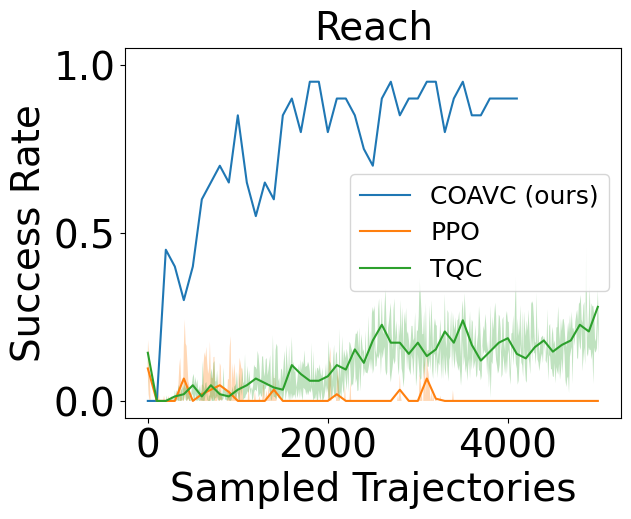
\includegraphics[width=\textwidth]{images/dense_1_big_font/Reach.png}
      \caption{One expert demonstration.}
    \end{subfigure}
    \begin{subfigure}[t]{0.32\textwidth}
      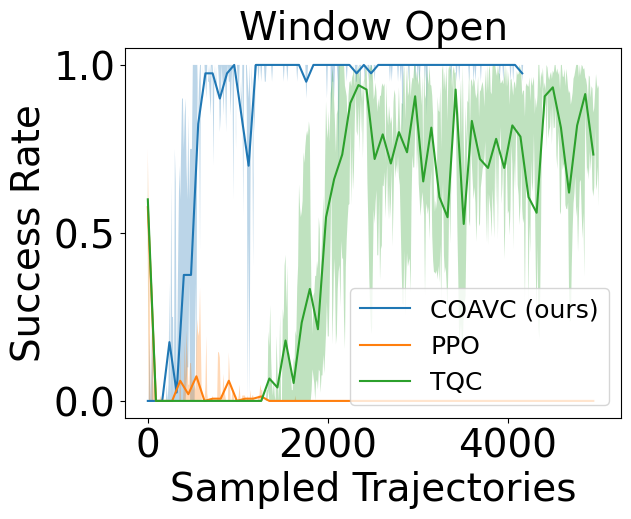
\includegraphics[width=\textwidth]{images/dense_1/Window Open.png}
      \caption{One expert demonstration.}
    \end{subfigure}
  
    \begin{subfigure}[t]{0.32\textwidth}
      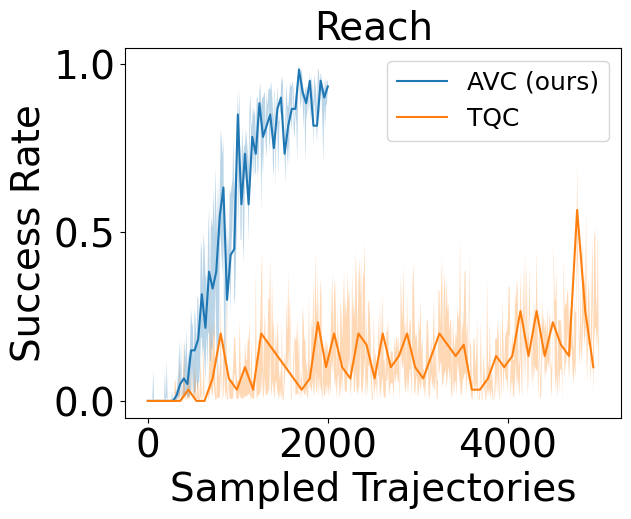
\includegraphics[width=\textwidth]{images/dense_0/Reach.png}
      \caption{No expert demonstrations.}
    \end{subfigure}
    \begin{subfigure}[t]{0.32\textwidth}
      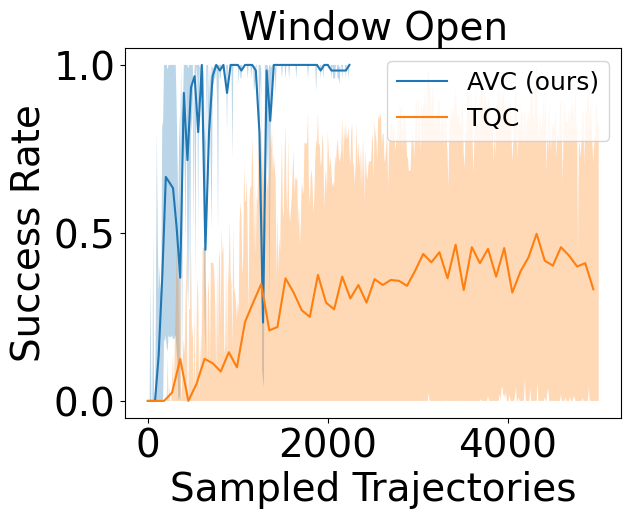
\includegraphics[width=\textwidth]{images/dense_0/Window Open.png}
      \caption{No expert demonstrations.}
    \end{subfigure}
    \begin{subfigure}[t]{0.32\textwidth}
      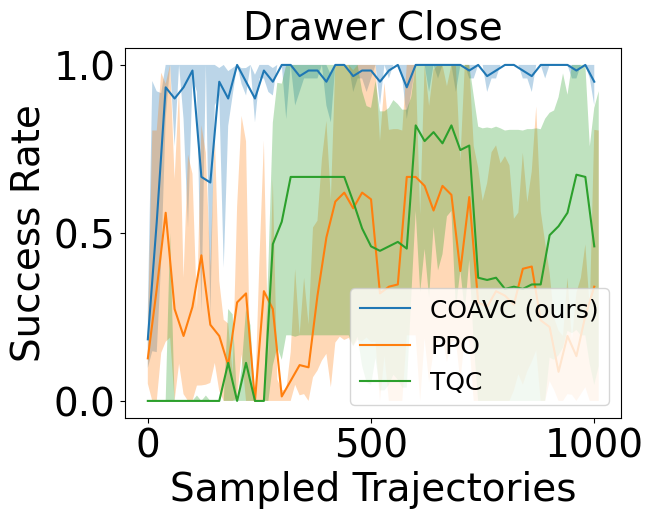
\includegraphics[width=\textwidth]{images/dense_0/Drawer Close.png}
      \caption{No expert demonstrations.}
    \end{subfigure}

  \end{figure}


\end{document}
